\documentclass{chi2009}
\usepackage{times}
\usepackage{url}
\usepackage{graphics}
\usepackage{color}
\usepackage[pdftex]{hyperref}
\hypersetup{%
pdftitle={Your Title},
pdfauthor={Your Authors},
pdfkeywords={your keywords},
bookmarksnumbered,
pdfstartview={FitH},
colorlinks,
citecolor=black,
filecolor=black,
linkcolor=black,
urlcolor=black,
breaklinks=true,
}
\newcommand{\comment}[1]{}
\definecolor{Orange}{rgb}{1,0.5,0}
\newcommand{\todo}[1]{\textsf{\textbf{\textcolor{Orange}{[[#1]]}}}}

\pagenumbering{arabic}  % Arabic page numbers for submission.  Remove this line to eliminate page numbers for the camera ready copy

\begin{document}
% to make various LaTeX processors do the right thing with page size
\special{papersize=8.5in,11in}
\setlength{\paperheight}{11in}
\setlength{\paperwidth}{8.5in}
\setlength{\pdfpageheight}{\paperheight}
\setlength{\pdfpagewidth}{\paperwidth}

% use this command to override the default ACM copyright statement 
% (e.g. for preprints). Remove for camera ready copy.
\toappear{Submitted for review to CHI 2009.}

\title{ drawnTogether -- a collaborative approach to virtual graffiti }
\numberofauthors{3}
\author{
  \alignauthor Jeremy Kelley\\
    \affaddr{Texas A\&M University}\\
    \affaddr{College Station, TX 77843}\\
    \email{jeremyk@tamu.edu}
  \alignauthor Kyumin Lee\\
    \affaddr{Texas A\&M University}\\
    \affaddr{College Station, TX 77843}\\
    \email{kyumin@cse.tamu.edu}
  \alignauthor Xiheng Zhang\\
    \affaddr{Texas A\&M University}\\
    \affaddr{College Station, TX 77843}\\
    \email{@cse.tamu.edu}
}

\maketitle

\begin{abstract}
In this paper, we propose and implement a new application enabling ubiquitous
creation of virtual graffiti, intended to support location awareness and
interaction amongst mobile people despite their lack of temporal co-location.
In particular, we developed a mobile application using the GPS and compass
within the iPhone 3G S to allow participants to create sketches attached to
real world geographic locations and others to view them and contribute at a
later time.  We intend to show user interaction rates among participants
increasing when they can contribute to something permanently, even in the
digital sense.
\end{abstract}

\keywords{put author keywords here} 

\category{H.5.2}{Information Interfaces and Presentation}{Miscellaneous}[Optional sub-category]

\section{Introduction}


\section{Approach}
We are going to develop a collaborative artistic application for the iPhone 3GS. This application allows users raw sketches on their iPhone and upload the sketch as well as their global position and orientation at that moment, to a server. The sketch can be anything the user wants to draw. It can be the view he/she is seeing, or the idea he/she is thinking about, or his mood and his feeling. The purpose of this application is to help users collaborate and communicate better with others in the same network, or let actors be more aware of what happened around based on context information and more involved in social activities. The context information contains both temporal and spatial information. Each sketch will be timestamped at the point it is uploaded to the server.

The spatial data has:
\begin{enumerate}
\item the current position the user locates, indicated by x (latitude), y
	(longitude) and z (altitude) available via GPS in the device.
\item the current orientation the user faces available via the magnetic compass
	within the device.  
\end{enumerate}

The orientation is important because view would be affected given different
orientation.

\begin{figure}
\centering
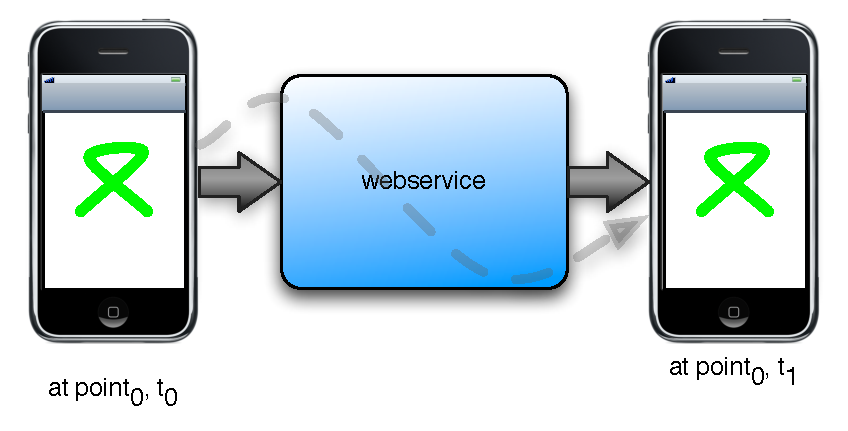
\includegraphics[width=.45\textwidth]{arch.pdf}
\caption{A simplified diagram showing client communications}
\label{fig:arch}
\end{figure}

Just like common social networks, users have his/her own networks in our
system. i.e., one may only interested in his/her friends' sketches or sketches
based on their tagged metadata.  It is expected that the amount of created
sketches could quickly overload our small interface.  For this reason, we are
initially allowing sketches to be filtered based on tags and their creator, as
seen in Figure \ref{fig:settings}.  Further work will focuse on ways to display
this potentially large dataset in a way optimized for small devices.

\begin{figure}
\centering
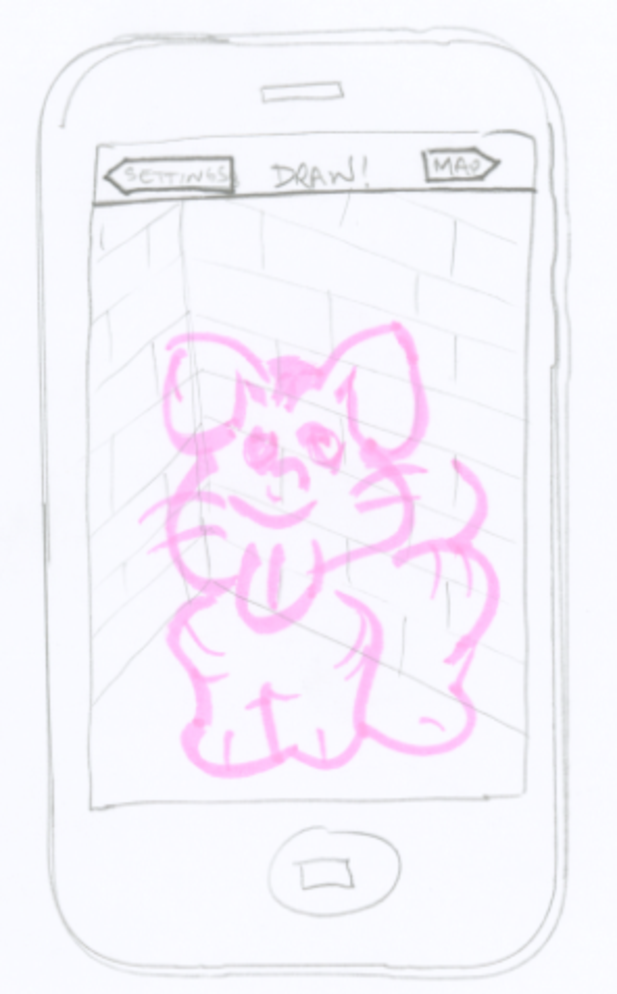
\includegraphics[width=.35\textwidth]{draw.pdf}
\caption{A mockup of the proposed drawing interface}
\label{fig:draw}
\end{figure}

\begin{figure}
\centering
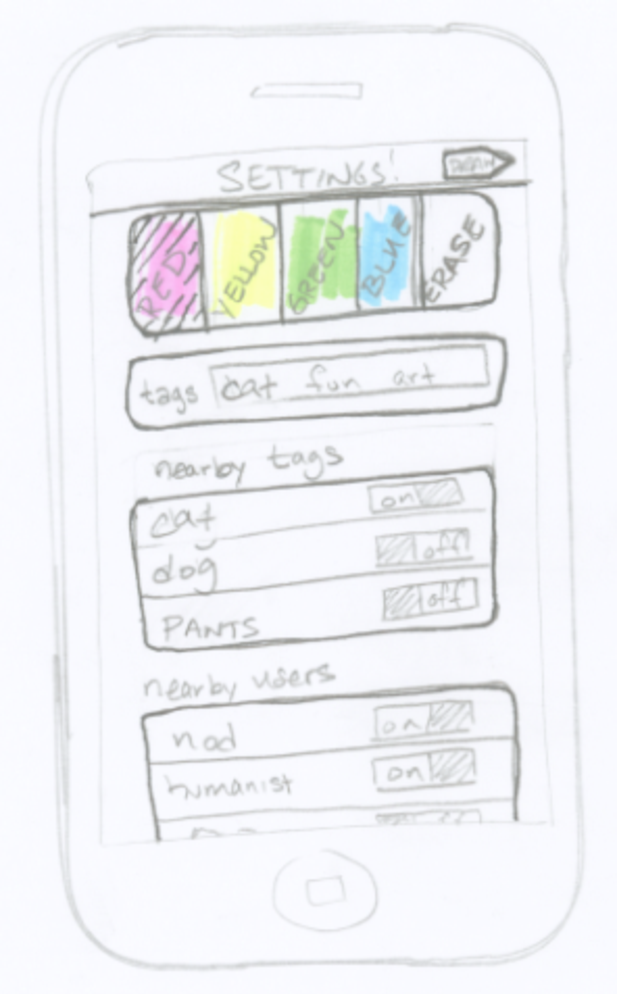
\includegraphics[width=.3\textwidth]{settings.pdf}
\caption{A mockup of the proposed settings interface}
\label{fig:settings}
\end{figure}

The specific activities users will conduct using our system include:
\begin{enumerate}
\item Hold iphone in hand, stay at any location GPS can track.
\item On the iphone screen, make some sketch as seen in Figure \ref{fig:draw}
\item For sketch, users can paint in a limited number of colors and have that
	creation tagged as seen in Figure \ref{fig:settings}
\item As the sketch is created, it will be uploaded to the server at small
	increments (every $n$ seconds)
\item Users can retrieve entries based on a simple query interface. Thus
	conditions involve: social relations, tag, time, and present location.
\item Users can view which sketches are near them via a map interface, as seen
	in Figure \ref{fig:map}
\end{enumerate}

Here is an initial description of the components we will need to prototype for
the system (hardware and software)

\begin{figure}
\centering
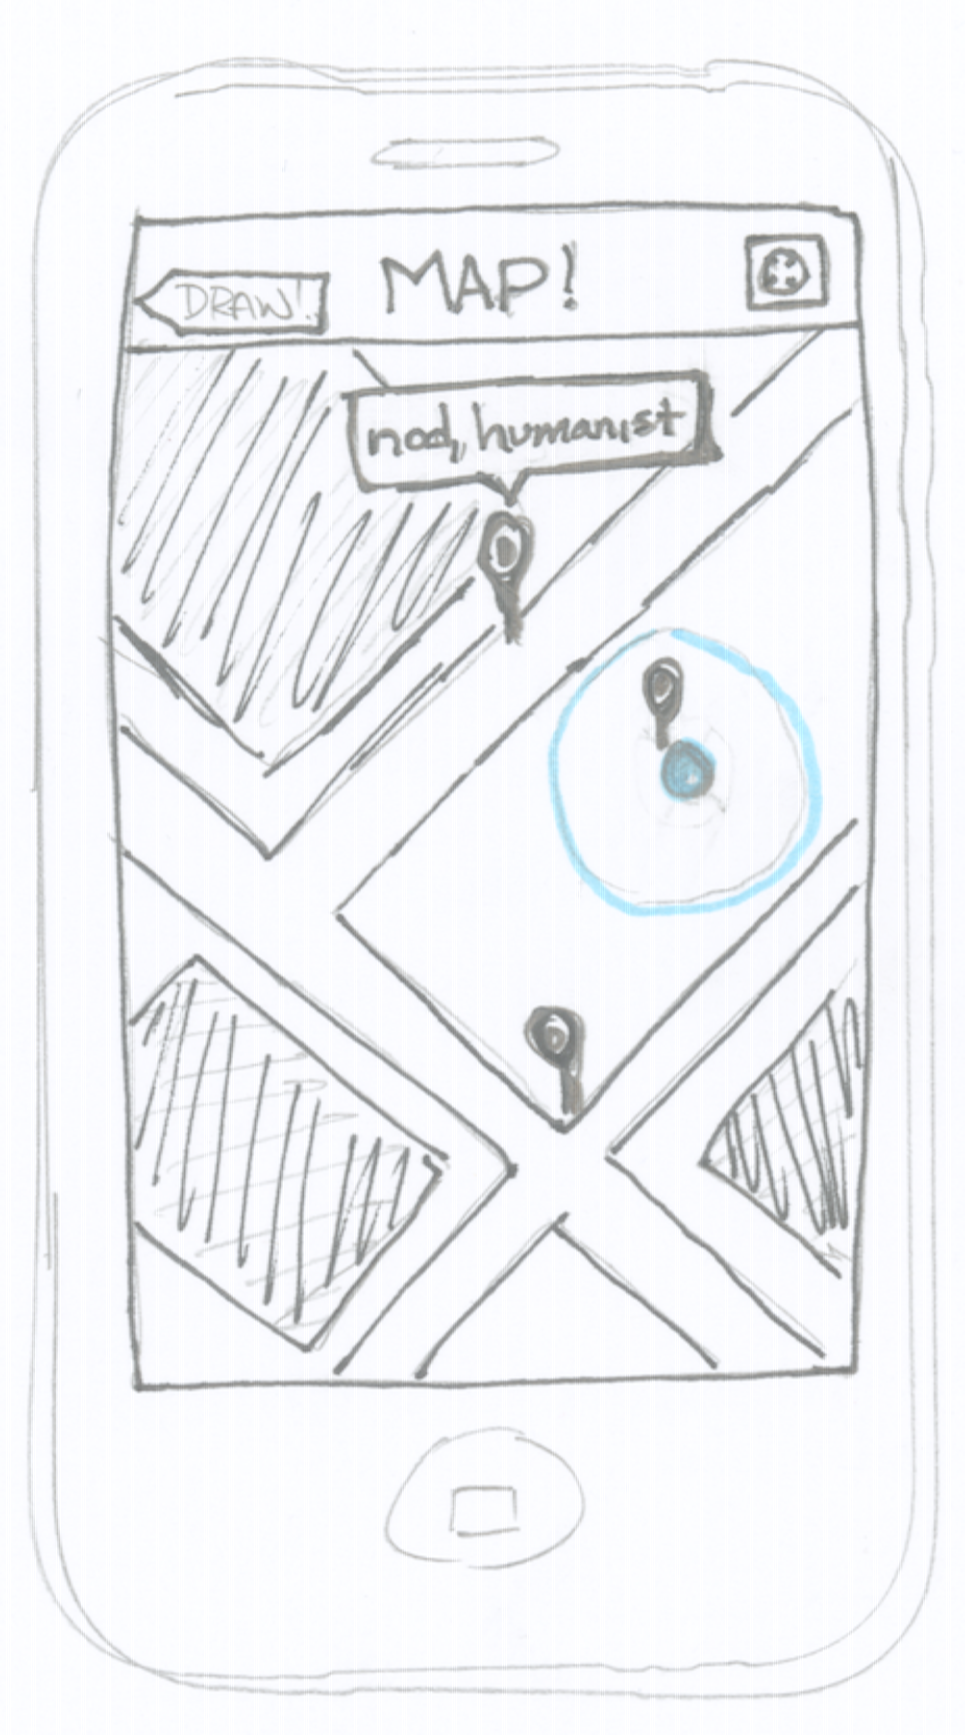
\includegraphics[width=.3\textwidth]{map.pdf}
\caption{A mockup of the proposed map interface}
\label{fig:map}
\end{figure}

\begin{enumerate}
\item Client interface
        \begin{itemize}
        \item iPhone 3GS
        \item  Sketch application
        \end{itemize}

\item Web service
        \begin{itemize}
        \item Operating system: Linux
        \item Web server: Lighttpd
        \item Web application: custom service build using Django framework
        \item Database: MySQL
        \item Code management tool during development: git
        \end{itemize}
\end{enumerate}



\section{design process}

\subsection{Ethnographic data gathering}
We conducted three semi-structured interviews and carried out at least five
other free form conversations around the goals of the project.  Since graphics
creation on mobile devices is very infantile, we instead chose to focus on
``normal users'' that may have used graphics programs and the intersection with
their mobile usage.

The three researchers in this project were to each speak with individuals and
gather information concerning artistic leanings and computer based tools used
in these endeavors.  In hindsight, we should have either had one individual
conduct all interviews, or provided a more rigid script for each interviewer to
use.  The questions started from the following set, but would often stray into
other tangents concerning the topic:

\begin{itemize}
\item Can you list any devices you have used for drawing besides paper?
\item Have you used any drawing software before?
	\begin{itemize}
	\item If yes, which tool have you used and how often have you used it? 
	\item Would you choose to use Paint or Photoshop if familiar with both?
	\end{itemize}
\item Do you prefer art creation on paper or via digital means?  Why?
\item Have you ever considered collaborating with others when creating artistic works?
\item Imagine you are able to draw on a screen and have that work appear on a
	building.  What would you draw?
\end{itemize}

These questions, although not rigidly adhered to, provided for interesting
conversation starters and were definitely useful in showing a definite interest
in our eventual application.

One of the interviewees came from China and is a student at Texas A\&M
University.  He mentioned he usually uses Paint application and sometimes uses
Photoshop and that, overall, he uses graphics applications about once a month.
His responses indicated that the MS Paint application is simple and easy to
use, and that Photoshop has too many functions and is quite sophisticated to
use.  Additionally, after he heard about our application, he said it would be
helpful to provide a function to search a sketch drawn by friends without going
to a certain location.

One of a the respondents, an economics student of Chinese origins, has never used an
iPhone before.  Yet, she is very interested in drawing and painting.  She
mentioned highly enjoying drawing on a small toy board which has an eraser as 
a child.  She randomly uses the Windows Paint application, as well.  Most often
though, she uses analysis software, such as SPSS to draw professional diagrams.
When questioned about pure artistic endeavors, she expressed a high preference
pen and a paper drawing and a complete disdain for using a mouse to draw strokes
when sketching. Her response concerning this area was ``If I can have a pen to
draw on the computer screen, I would definitely draw a good picture.''
Concerning collaboration, she definitely showed some excitable interest but her
biggest concern was the ability to tell her strokes apart from others.   When
the question about drawing on a screen and appearing on a building was
broached, she replied that she would like to draw something related to her
surroundings and that she would care about others sketches.  In particular, she
remarked, ``That's one aspect of collaboration, right? First, I care about my
friends' drawing. Then people who share the same interests with me.'' 
When our intended application was finally revealed, she said she would care
more about what people around her were drawing.

Another interviewee, a technology worker from Houston, TX, mentioned being
highly proficient in multiple graphics applications, including Photoshop.
Throughout the interview, his mind raced with different ways to collaborate on
different projects even at one point asking ``Would it be possible to really
project what others were drawing onto an external wall for live events and
concerts?''  This was an idea previously not considered by the researchers and
one that is being heavily considered as a way of involving passersby who may
not have a device but could still be considered consumers of collaborative
creations.

\subsection{Storyboards}
We can apply our application to various scenarios. In this section, we show two
of them.  Storyboards for the intended applicaiton 

\subsubsection{Scenario 1: collaborative drawing}

Alice and Bob are students at Texas A\&M University and are friends. Alice
wanted to draw the MSC building before it is remodeled, so she went near to the
building and sketched it using our application. She did not finish the drawing
because of a class. While she is going to a classroom, she sends a SMS message
to Bob. The message is ``Could you finish the sketch for the MSC building in
location X?'' Fortunately, he is passing in front of the building and starts to
add some sketch into the figure, which Alice drew. Sometimes later, he finishes
to draw the building and sends a SMS message to her. The message is ``I'm
done!'' After the class is finished, she goes to the location in which she drew
the building. She can view what they drew and is satisfied about what they did.
This can be weakly seen in Figure \ref{fig:s1}.

\subsubsection{scenario 2: event impressions}

Alice and Bob can attend a public event, such as a conference or a concert.
While at the event, each user contributes small sketches to the location.  On a
whim, Alice decides to draw the standing position of each speaker during their
talk or show and tags these creations as ``position''.  Likewise, Bob decides
that each time a question is asked from the audience, he will annotate that by
creating a mark on the screen and tagging it ``question''.  At the end of the
conference, they each view the other's visual notes and deduce several
anecdotal observations related to audience participation and performer
position.  This can be weakly seen in Figure \ref{fig:s2}.

\begin{figure}
\centering
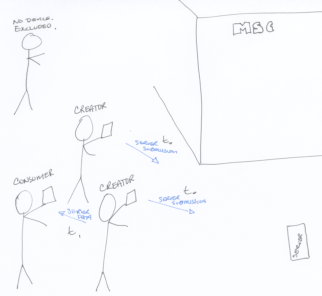
\includegraphics[width=.50\textwidth]{scen1.pdf}
\caption{Scenario 1} \label{fig:s1}
\end{figure}

\begin{figure*}
\centering
\includegraphics[width=.80\textwidth]{scen2.pdf}
\caption{Scenario 2} \label{fig:s2}
\end{figure*}



\section{User Study 1}
\subsection{Interviewees}
We conducted nine people:

\begin{itemize}
\item (A) male, an iphone 3G S user
\item (B) male, a computer science graduate student
\item (C) female, a person who enjoys drawing
\item (D) male, an iPhone 3G S user
\item (E) male, a computer science graduate student
\item (F) male, a computer science graduate student
\item (G) male, professional graphic artist and iPhone 3G S user
\item (H) female, non-technical profession, non-iPhone user
\end{itemize}

\subsection{conducting user study}

Conducting the user study can involve multiple methods.  For our study, we took
an informal, guided conversational approach to gather the information.  We
provided a semi-structured questionnaire that our interviewers were to follow.

This questionnaire was divided up into multiple phases.

\subsubsection{ Introduction }

This phase consists of multiple steps:
\begin{itemize}
\item welcome and greetings
\item gather consent and completion of form
\item introduce the system in conversational form
\item communicate goals for this study
\end{itemize}

This phase is general housekeeping and provides for a welcoming and
customization period between the interviewer and interviewee.  Any general
questions are encouraged at this point about the general concept, but the
system has not been officially ``placed in their hands'' yet.

\subsection{Facilitation}

In order gather information about usage, we will physically hand the users a
lo-fi representation of the drawnTogether interface in the form of a tangible,
translucent enclosure with cards that can swap out to represent the varying
views of the application.  When the user ``navigates'' between the views, the
interviewer will act as the computer and move the cards for the user.  The
benefits of this are numerous, but primarily, it allows us to iteratively
improve the interface and pilot new versions in a much faster way than
implementing the changes in software first.

We interviewed multiple individuals (eight total) over a period of three days.
The first six individuals used the same version of our interface.  The last two
used a modified version based on feedback gained from earlier interviews.  The
second version of our application views were very well received, as will be
seen in the following commentary.

For each interview, we began our questions with handing them the device, then
asking the following:
\begin{quote}
Is there anything particularly interesting about the concept of the
application?
\end{quote}

Most respondents actually felt the application to be quite interesting.
Respondent B, however, felt that it's merely a ``funny application'', and doubted if 
there would be enough situations for the system to be used.   He did provide
one possible  scenario. Imagine a group of architecture students
enter into one building to make a sketch of the inside structure of this
building. Each student can find whether the viewer around him or her has been
drawn or not. If not, he can add his sketch on the screen of the application.
If yes, he may ignore it and go to other places to draw or make some correction
based on others' drawings.  It was interesting to the researchers that even a
skeptic began to imagine practical, unforeseen collaborative uses.

Following the initial question, we followed with providing four erasable
markers of differing colors to the interviewee.  We had them ``navigate'' to
the drawing screen if he or she were on a different screen.  At this point, we
asked the following:

\begin{quote}
Can you draw a simple picture using multiple colors on the screen?
\end{quote}

With this question, we wanted to gauge the intuitiveness of the interface and
the user's ability to recognize visual affordances and their mapping to
intended tasks.  Person A asked ``Can I draw now?  What's the status of my
pen?''.  Several users touched the settings button before ever trying to draw,
with the purpose of exploring their options and tools before actually beginning
any sketch creation.  Person C immediately picked up a random pen (blue) and
began drawing on the screen.  When asked how they would change colors in the
application, the response was ``Oh\ldots  the settings page'', to which she
instantly and easily navigated to the page and chose the blue color.  Again,
with each navigation, the interviewer acted as the computer and moved the cards
as requested to transfer the user to different views.  Once in the setting
page, all users had an apparently clear understanding of how to manipulate the
current drawing color or erasure.

Multiple users asked about the tagging features visible on the settings page.
With minimal instruction from our facilitator, users understood the nature.
One thing was made clear to the developers with these questions, though.  The
ability to create tags and filter tags on the same view was a little confusing
and needs to be revisited.  The later revision used by the last two
interviewees provided a much clearer mapping and helped to eradicate most of
the confusion.

There were several questions about the appropriate time to tag a drawing or as
to the origin of the tags used for filtering.  These questions were quite
helpful in illuminating deficiencies with some of the feedback mechanisms
around the affordances related to tagging.

One interesting suggestion from multiple users was to add a voting feature for
a given location's sketches.  This way, a ranking per location could be used to
sort each location and be communicated on the map also.

Our next question was one which encouraged them to examine the map view, if
they had already not seen it:

\begin{quote}
Please navigate to the map view. {\it [pause for navigation]}
What pieces of information do you gather from this view?
\end{quote}

Once on the map, Person G mentioned ``Oh, I can see where other users sketches
are.  Cool''.  This was very satisfying to the researcher that the primary and
immediate purpose of the map was summed up so well.  User A asked, ``Can you 
show the sketches actual sketches from different locations on the map? In a
pop-up window?''


\subsection{Interview Completion}

In this phase, we attempted to provide a summary of each person's response and
to gather further clarification if needed.

We also ended with one final question, intended to spark a free form conversation:

\begin{quote}
Are there any recommendations you would make to improve your experience?
\end{quote}

Two individuals suggested moving the color palette from the setting page to the
bottom of the drawing view.  This would have the effect of drastically reducing
the interaction required for a meta task of changing the drawing color.  Several
users changed colors at least twice, so the benefits of this change seem
beneficial.  For the final two interviews, this change was adopted and proven
to be a valid enhancement immediately.  Person G used the modified drawing view
and changed colors five times while creating a sketch.  Person H changed colors
four times.  This was a definite, measurable improvement and allowed for a more
refined workflow for task completion.

The sacrifice of reduced drawing area was mitigated by removing the top bar
completely in the drawing view and adding navigational elements to the bottom
toolbar to allow for access to settings and the map.  This had no visible,
negative effect on the latter participants in the study on their ability to
navigate between views.

Another suggestion, offered by Person A, was to launch the application with the
map page initially.  Further conversation with the participant on this
consideration showed several potential benefits of adopting this.
\begin{itemize}
\item Participation feedback is immediately communicated by this macro approach
to making visible the locations containing sketches.  Each sketch becomes just
one minor data point on the geographical plot.
\item Users can immediately choose to change their location in order to either
add to an existing drawing or to create something new and unique
\item Community involvement is augmented by seeing participation.  If each map
pin is somehow annotated with the sketch age, a visual component could easily
communicate a temporal nature for each sketch showing which areas could benefit
from a ``fresh creation''.
\end{itemize}

In closing, almost all participants expressed an interest in getting this
application for their personal use.  



\section{Implementation}

The scope of this project and the tight deadlines means that team communication
and productivity is of the utmost importance.

\subsection{ Application Environment and Development Tools }

\subsubsection{ Mobile Client }

Since the prototype is intended for the iPhone OS, there are few options for
development environments.  The path of least resistance (and greatest
productivity) is for the application to be written in Objective C, and built
using Apple's iPhone SDK toolchain integrated into the Xcode IDE.  It is
possible to develop iPhone applications outside of Xcode, using other text
editors and foregoing the builtin debugging integration that Xcode offers, but
to compile and link, one is still required to use the provided tools by Apple.
For this reason, our team will focus on the Xcode environment and the full
stack that it has to offer.  In particular, we will be using the following:

\begin{itemize}
\item development workstations will run OSX
\item Xcode
\item iPhone 3G S
\item iPhone Simulator
\end{itemize}

\subsubsection{ Web Service }

In order for the applications on the client devices to share content, a
centralized web service is required.  There are many options within this realm,
however, for ease of development since time is short on this prototype, this
web service will be built using the following:

\begin{itemize}
\item Python scripting language
\item Django Web Framework
\item Lighttpd HTTP Server
\item MySQL Database
\item JSON for data transport
\end{itemize}

This stack of tools has been widely utilized in numerous installations and in
particular, the Python language has proven itself to be quite powerful, yet
easy to learn.

\subsubsection{ Version Control \& Source Code Management }

In order to facilitate sharing our work, we have created a repository at
GitHub\footnote{http://github.com}.  This allows us to use Git, a distributed
version control system, for all of our created content.  Our source code,
scripts, and even our papers (written in \LaTeX) will be stored in this shared
repository.  This allows us, as a distributed team working in disparate
locations, to share all content and stay up-to-date with others contributions.

Git also provides issue tracking that we have begun using in an effort to track
progress and discussion on multiple concurrent items.

\subsection{ Development Milestones  }

\begin{itemize}
\item 17 Nov -- Storyboards and Lo-fi Prototypes
\item 19 Nov -- Webservice completed and API locked for data transfer
\item 23 Nov -- pre-Alpha ``Sketchable'' interface working on Sim with fabricated geo data
\item 24 Nov -- Initial User Feedback incorporated into final designs
\item 26 Nov -- Early ``Alpha'' version of the mobile client ready
\item 1 Dec -- Prototype due

\end{itemize}

\subsection{ Application Architecture }

The heart of the mobile application will be the integration of a live video
feed from the device's camera overlaid by user contributed sketches for the
current location of the device.  The application will rely on Apple's
CoreLocation service to provide the location and orientation information in
order to retrieve user content from the web service.  We will run an NSTimer
that will create NSInvocationOperations at regular intervals to submit any user
created content in the background during viewing and to retrieve any new
content for the user's current geographic area.

We intend to incorporate a simple user identity component using Twitter.  This
will allow us to attach a user to a sketch without having to manage the
identity infrastructure.  By having identity information attached to each
contribution, we will also have the ability to allow users to filter based upon
the user.

There will be a tagging component, although it will be limited in this initial
prototype.  The user will be able to create a set of tags that will be applied
to sketches created after tag assignment.

Finally, a map view will be provided which will indicate to the user sketches
near to them, to allow for ``sketch tours'' or other artistic discoveries.

\section{evaluation}

\section{prior work}
Zurita et al. \cite{sketching:zurita} presents MCSketcher, a mobile
collaborative sketching system, using handheld devices in an ad-hoc network.
People can draw sketches with collaborators in the same page in the system.
They can take a picture and use it in the background of the drawing. The system
supports gesture recognition for basic navigation gestures, and selecting and
resizing items. Collaborative work is only available in an ad-hoc network. In
other words, friends or collaborator can only work together in close distance.
Our application connects to a server to store what users draw and to retrieve
what they drew in the past using cellular networks. One can collaborate with
not only friends, but also any people.

Kim and Dey \cite{augmented_reality:kim} presents displaying augmented reality
based car navigation information on windshield. Augmented reality helps elder
people can concentrate to drive a car and easily follow directions from a
navigation system. Augmented reality is one of ways to display various
information in a view. Likewise, overlapping sketches can help for users to
know what has happened in a certain location, even though augmented reality is
not exactly applied to our application. In addition, our application provides
users with some filters such as name of a drawer, time and so on, so that they
can select what they want to view.

Bast\'{e}a-Forte and Yen \cite{brainstorming:marcello} presents a collaborative
sketching tool. Each user has a Tablet PC to draw some sketches and to view
shared sketches. Each userÕs drawling is synchronized, so that users can view
the same drawling. The collaborative sketching tool helps each userÕs
contribution is equalized although it reduces total number of sketches. Our
application enables users to collaborate drawing no matter what their
relationship is.

The authors in \cite{context:weis} are trying to combine various context-aware
applications. They want to retrieve data from different sources and services,
thus design a general purpose client software that can be used to access a
variety of context-aware services. In their paper, they proposed an
architecture of their system model. They use messenger protocols. If a service
has new information, it sends a short notification message via the servers to
the client. The client can then decide whether it wants to retrieve the full
data. Therefore, the client can directly connect to the service. A discovery
service is used to find services which are relevant for a client in its current
context. It uses the messenger protocol to inform the client software about new
services. In our project, we will find sketches relevant for a client based on
its current context information - both GPS data and twitter friends.

 The authors in \cite{ink:lindell} tested a few hardware and software
technologies in real-time collaborative system, basically raised two
fundamental principles - collaboration and persistence. The two principles
refer to the ability to communicate ideas with other interested parties in
real-time and the ability to store the results of those interactions for
long-term reference, respectively. The softwares include NetMeeting, OneNote,
DyKnow. Their work is mainly to help students share class materiel and
simultaneously edit presentation text or  sketch.

\section{discussion}

\section{conclusion and future work}


\bibliographystyle{abbrv}
\bibliography{sample}

\end{document}
